\chapter{Conclusion}
 \section{Next-Generation Sequencing}
	A variety of sequencing platforms, software, and use-cases is present in sequencing experiments.
	In our study, we wanted to evaluate the transcriptomes of non-model species (i.e. species without a sequenced genome).
	At the time of the initial experimental design, 454 sequencing was the commonly favorited approach for sequencing non-model species.
	However, it remained unclear, whether \ac{OLC} or \ac{DBG} assemblers were more successful in assembling full-length contigs for each transcript.
	To find an answer to this question, we used the \species{Arabidopsis thaliana} genome as a well known reference.
	Besides, we were interested in evaluating the assumption\footnote{It really was just a guess, but I might need to call it hypothesis in my final version}: More reads lead to a better (i.e. more complete) assembly.
	From this reference we generated simulated 454 reads, based on actual sequencing data from former studies in \species{Cleome} \cite{op_Braeutigam2010}.
	These simulated reads were perfect in terms of sequencing errors.
	Therefore, we additionally created read libraries with artificial 1\%, 3\%, and 5\% base changes.
	With the 4 read libraries as input sequences, we used the assembly software: SOAP\cite{unknown}, Velvet\cite{unknown}, MIRA\cite{unknown}, CAP3\cite{unknown}, TGICL\cite{unknown}, and \cite{CLC}.
	Traditional quality parameters to assess a \foreignword{de novo} transcriptome assembly were taken from genome assembly.
	These metrics, namely N50, maximum contig length, number of contigs, describe the size and distribution of the contig library.
	As a rule of thumb, in genome assembly larger contigs represent a better assembly.
	In transcriptome assembly, however, this rule does not apply.
	A very long contig can result from the assembly of multiple genes.
	To describe the quality of an assembly in a less biased way, we used percentage of full-length transcript, i.e. the relative length of a contig to it's best hit reference gene's length.
	As a visualization we plotted number of reads used for the assembly against percentage of full-length transcript.
	
	With perfect reads in all assembly software the contigs with >200 reads were mostly 100\% assembled.
	However, in \ac{DBG} assemblers several transcripts did not get assembled more than 20\% - 60\% of the full-length transcript.
	We did not find this phenomenon in \ac{OLC}assemblers.
	Thus, we can conclude, that more reads make an assembly even worse, if using \ac{DBG} assemblers, but have no negative effect on \ac{OLC}assemblies.
	With increasing percentage of simulated sequencing errors (i.e. random base changes) the difference becomes less significant.
	
	%Hybrid transcripts: how many??? <-Connection to second publication
	
	When using cheaper and less error prone Illumina sequencing, the numbers of reads one sequencing run yields increases drastically.
	Thus, \ac{OLC} assemblers are not feasible if at all able to assemble the reads in terms of computational power.
	Yet, the number of transcriptome sequencing experiments in the public databases and the variety of used assembly software are increasing.
	As already showed, assembly algorithms are highly sensitive to uncontrollable changes in the sequencing experiment.
	To cope with this, we set a standard quality assessment approach.
	The aim was making public datasets more accessible to other working groups by providing additional information along with the sequences.
	These information do not alter nor improve the assembly quality, but they allow for a reliable quality estimate.
	Hence, a comparison of sequencing experiments can be investigated based on the quality parameters.
	
	The quality assessment parameters we suggest:
		
		\begin{itemize}
			\item number of contigs
			\item N50 of contigs
			\item Venn diagram of contigs mapping and reads mapping to reference gene
			\item percentage of contigs mapping to reference
			\item number of hybrid/chimeric contigs
			\item type of hybrids
			\begin{itemize}
				\item read-through reads of neighbouring genes
				\item fusion genes
			\end{itemize}
		\end{itemize}
		
		We tested all these parameters in an actual sequencing of Arabidopsis thaliana transcriptome against the Arabidopsis thaliana genome.
		Compared with the theoretical values for the aforementioned parameters the experiments showed us that we are still far from ideal assemblies.
		Yet, the suggested parameters allow for a rating of the completeness and reliability of the assembled transcriptome.
		Until now, there is no approach to detect chimeric contigs in transcriptome assemblies, that is independent of a reference genome.
		Thus, detecting chimeric contigs in a non-model species without a reference is not possible so far.
		An approach using expression information to identify the fusion positions did not succeed (figure \ref{fig:conclusions_chimeraByExpression}).
		A perfect assembly of the actual transcriptome might be possible with single molecule sequencing techniques, once practicable.
		
		\begin{figure}%
			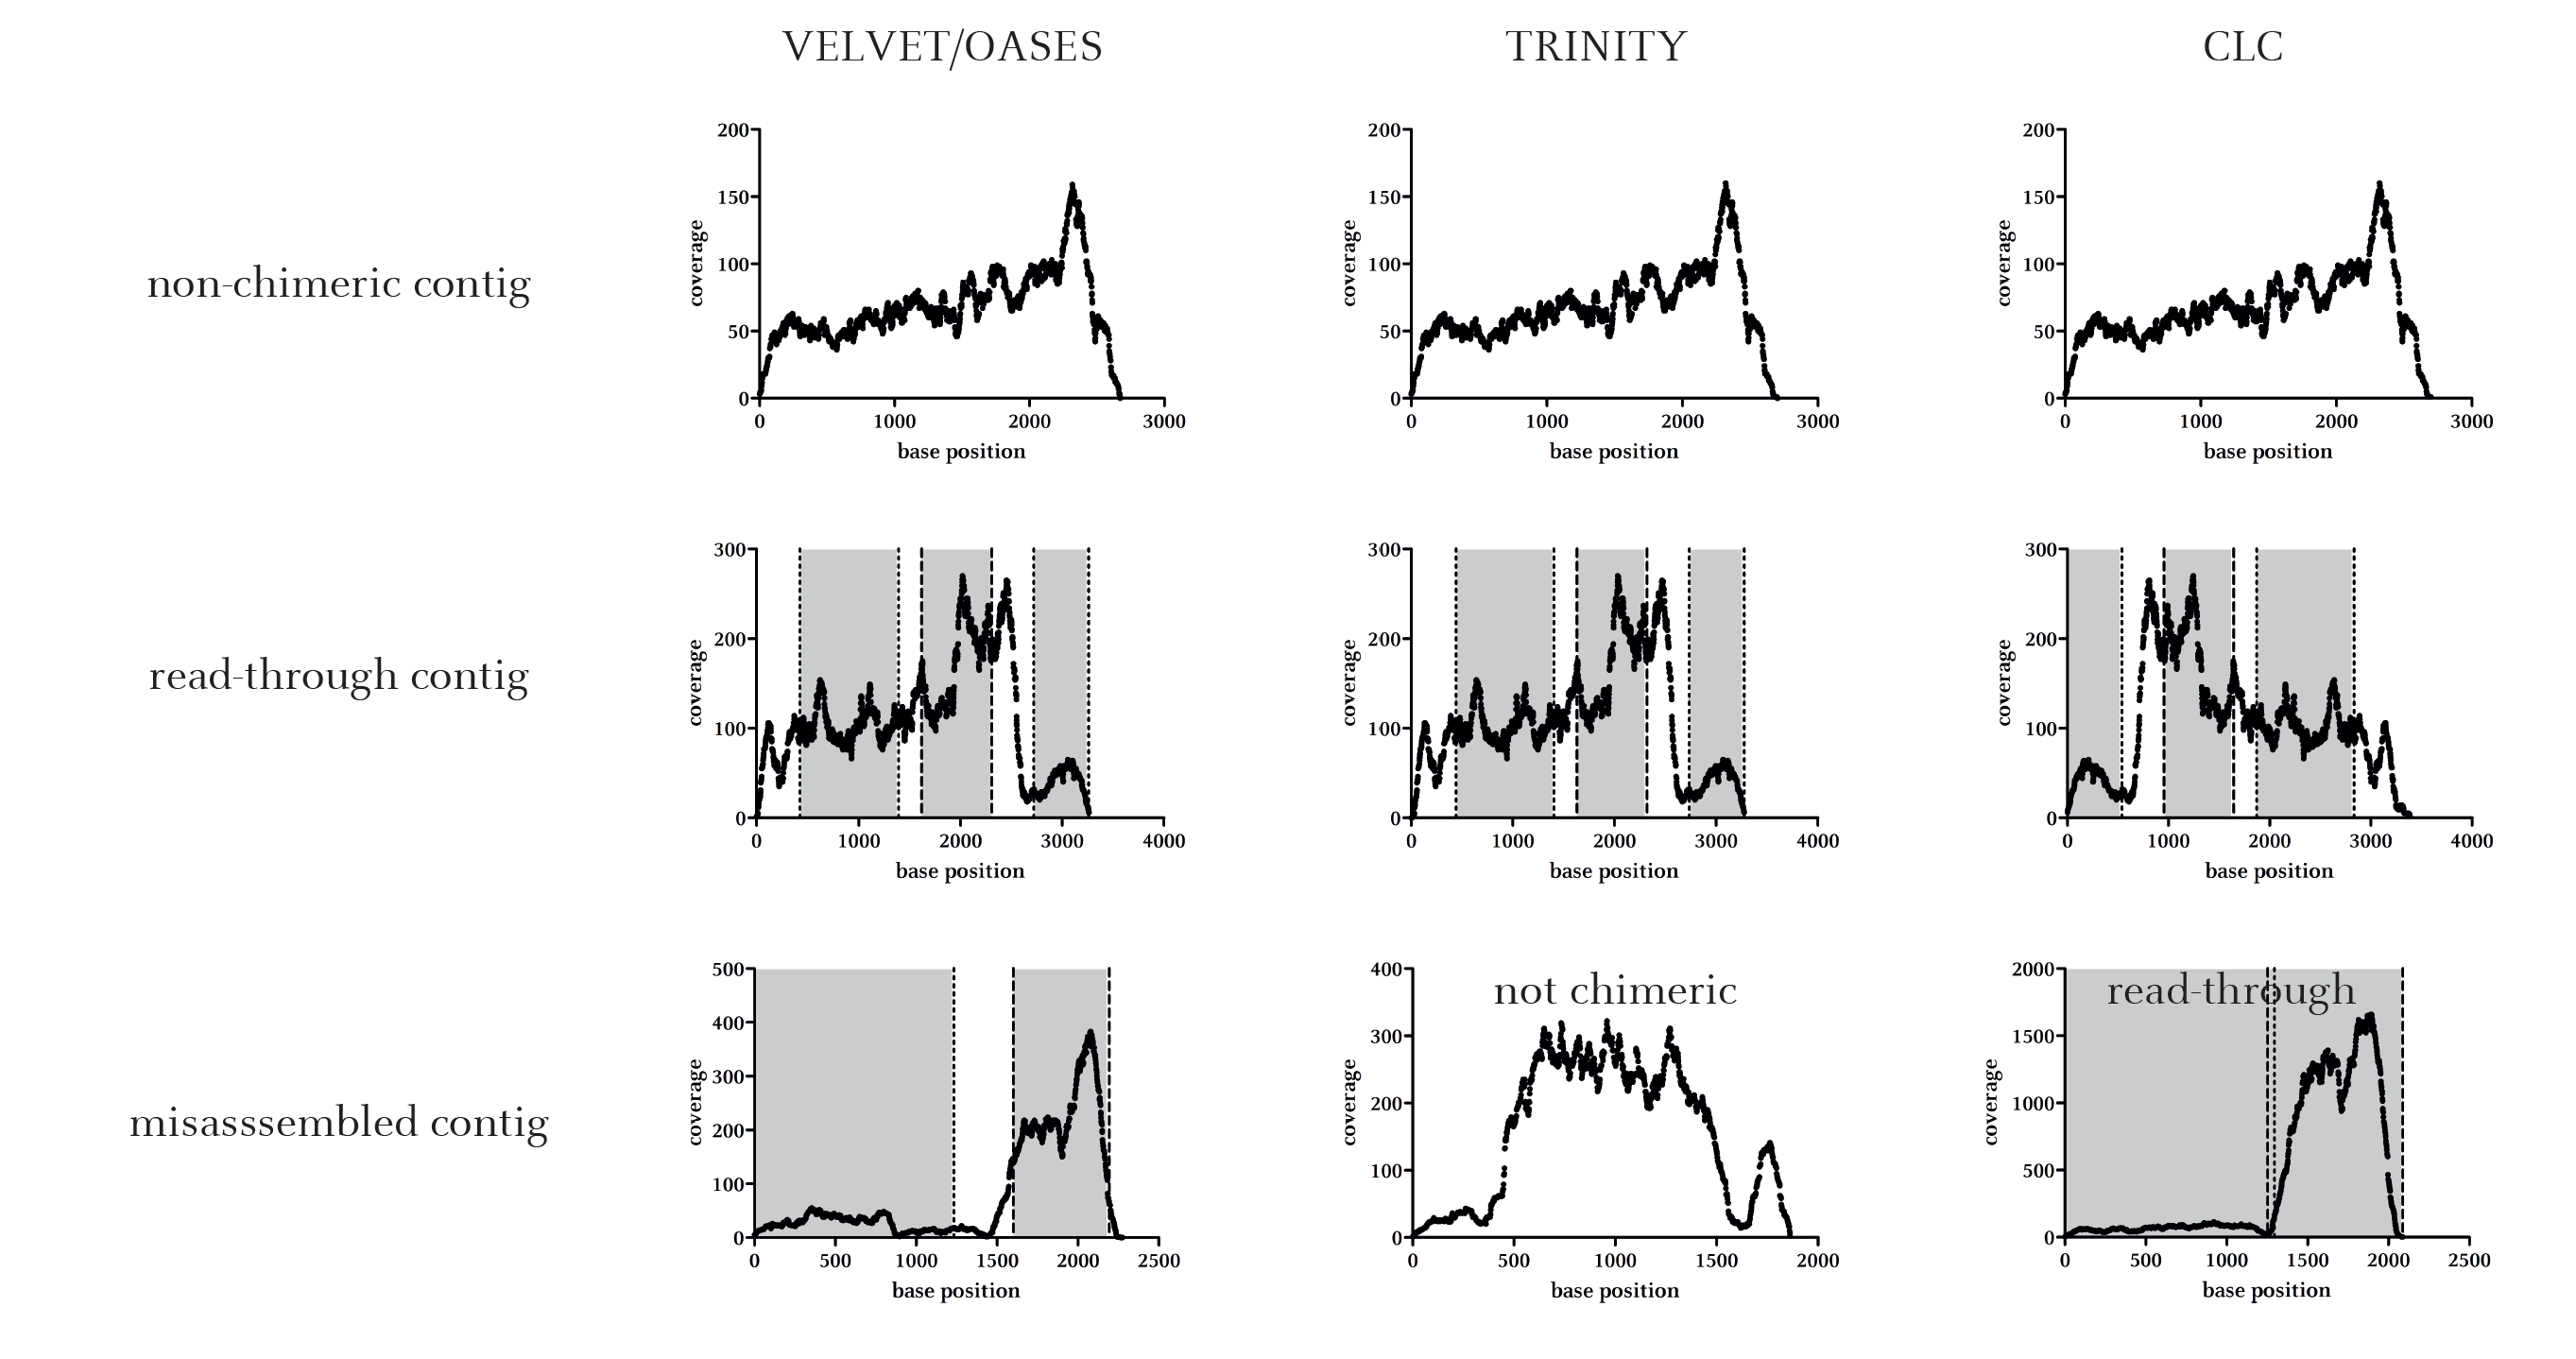
\includegraphics[width=\columnwidth]{images/conclusions_chimeraByExpression}%
			\caption{The read expression across chimeric genes does not reveal the positions of gene fusion marked by dashed lines (determined by mapping to reference genome). (This figure was presented as part of a poster on BioComp2012)}%
			\label{fig:conclusions_chimeraByExpression}%
		\end{figure}
	%Hybrid contigs, Contig and read mapping, 